\subsection{Построение архитектуры}
\label{sec:design:dev}

Сформулировав требоваяния к программному продукту, приступим к проектированию.

Необходимо определиться с методом преобразования адиозаписей к виду, который будет точно описывать композицию. Существует большая разница между характеристиками композиции, которые влияют на предпочтения пользователей, и характеристиками, которыми обладает сам сигнал. Поэтому работать непосредственно со звуковыми сигналами недостаточно эффективно, а так же достаточно долго. Спектрограммы ускоряют процесс работы, но так же не настолько эффективны, поскольку не учитывают особенности человеческого уха. Человеческое ухо, как говорилось ранее, воспринимает звук несколько иначе, что требует определенных корректировок. Для того, чтобы учесть поправки на восприятие звука ухом человека, можно отобразить спектрограмму на мел-шкалу. В результате мы получим мел-спектрограмму. Работать с мел-спектрограммой достаточно долго ввиду её большого размера. Необходимо найти способ сжать информацию до приемлемых размеров, при этом не потеряв в точности.

Для того, чтобы сжать информацию и учесть поправки на человеческое ухо, было решено использовать мел-частотные кепстральные коэффициенты.

Достоинства этого метода:
\begin{enumerate}
  \item используется спектр сигнала, что позволяет учесть волновую природу звука;
  \item спектр проецируется на мел-шкалу, что позволяет учесть восприятие частот человеческим ухом;
  \item возможность сжать количество информации количеством вычисляемых коэффициентов.
\end{enumerate}

Осталось понять, как преобразовать сигнал в набор коэффициентов. Первым делом нам нужен спектр исходного сигнала, который мы получаем с помощью преобразования Фурье. Для того, чтобы не потерять временную составляющую, воспользуемся оконным преобразованием Фурье. Теперь полученный спектр нам нужно расположить на мел-шкале. Для этого мы используем окна, равномерно расположенные на мел-оси (см. рисунок \ref{sec:design:dev:windows}).

Если перевести график, изображенный на рисунке \ref{sec:design:dev:windows}, в частотную \\шкалу, можно увидеть график, изображенный на рисунке \ref{sec:design:dev:windows_mel}.

\begin{figure}[h]
\centering
	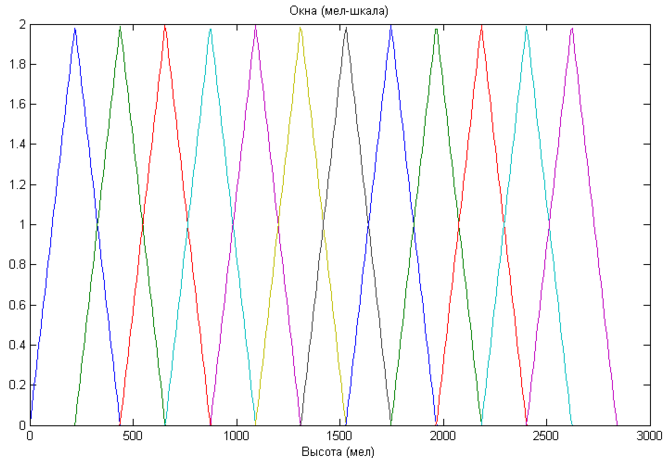
\includegraphics[scale=0.68]{windows_mel.png}
	\caption{Окна на мел оси}
	\label{sec:design:dev:windows}
\end{figure}

\begin{figure}[h]
\centering
	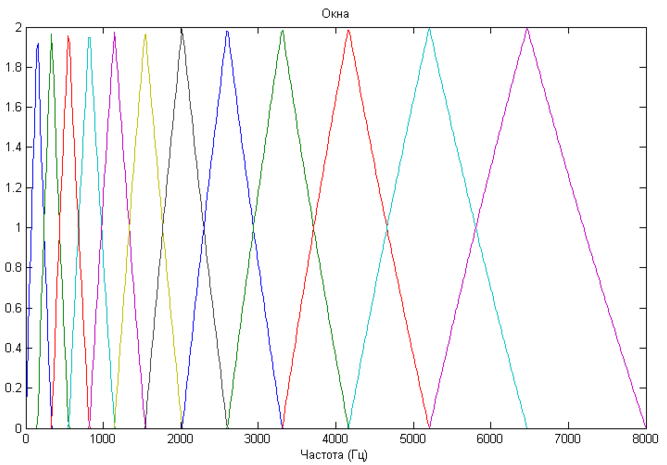
\includegraphics[scale=0.68]{windows_hz.png}
	\caption{Окна на мел оси, переведенные в частотную шкалу}
	\label{sec:design:dev:windows_mel}
\end{figure}

На этом графике заметно, что окна «собираются» в области низких частот, обеспечивая более высокое «разрешение» там, где оно необходимо для извлечения. Простым перемножением векторов спектра сигнала и оконной функции найдем энергию сигнала, которая попадает в каждое из окон анализа. Мы получили некоторый набор коэффициентов, но это еще не те коэффициенты, которые мы ищем. Пока их можно было бы назвать мел-частотными спектральными коэффициентами. Возводим их в квадрат и логарифмируем. Нам осталось только получить из них кепстральные, или «спектр спектра». Для этого мы могли бы еще раз применить преобразование Фурье, но лучше использовать дискретное косинусное преобразование.

Таким образом мы имеем очень небольшой набор значений, который при извлечении успешно заменяет тысячи отсчетов речевого сигнала.

Преобразовав сигнал, необходимо создать инструмент, который будет извлекать характеристики из полученных данных. Для этого решено использовать методы, основанные на машинном обучении. Для того, чтобы применять машинное обучение, необходимо построить модель, которая будет являться искомым инструментом. Для построения модели необходимо разработать структуру модели, а так же выбрать библиотеку для обучения.

В качестве библиотеки для обучения была выбрана TensorFlow от компании Google. Она предоставляет большой набор инструментов, при помощи которых можно обучать модели на различных системах. Так же TensorFlow помогает работать с высокой степенью оптимизации, что ускоряет процесс обучения и обработки данных.

Для того, чтобы ускорить процесс прототипирования и повысить уровень абстракции, поверх TensorFlow будет использоваться библиотека Keras.

Связка Keras -- TensorFlow позволит оптимально расходовать ресурсы системы, на которых будет запускаться сервис, при этом будет сохранен высокий уровень абстракции, что повысит читабельность и универсальность кода.

Построим архитектуру модели, которая будет извлекать высокоуровневые характеристики из музыкальных композиций. Для извлечения признаков хорошо себя показывают глубинные нейронные сети. Для извлечения признаков из матриц больших размерностей, к которым относится полученный список мел-кепстральных коэффициентов, лучше всего использовать сверточные нейронные сети. Но для извлечения временных паттернов лучше всего себя зарекомендовали рекуррентные нейронные сети. Для получения наилучшего результата, скомбинируем сверточные нейронные сети и рекуррентные нейронные сети в глубинной нейронной сети. В результате получим нейронную сеть, в которой будет 6 слоев (см. рисунок \ref{sec:design:dev:neuralnet}). Первые 4 слоя являются четырехслойной сверточной нейронной сетью, которая будет извлекать локальные признаки. Следующие 2 слоя являются двухслойной рекуррентной нейронной сетью, которая предназначена для агреггирования временных шаблонов. Это более эффективный подход, чем, например, использовать усреднение результатов.

Полученная нейронная сеть может быть больших размеров. Для того, чтобы сократить время на загрузку нейронной сети из дискового пространства в память, следует держать сеть в оперативной памяти. Наиболее эффективно хранить сеть в отдельном процессе, в который будут поступать данные для обработки. Это снизит затраты по памяти, а так же позволит обрабатывать большее количество данных за единицу времени. Процесс, который хранит и использует нейронную сеть, решено реализовать в виде демона.

Для того, чтобы предоставить API, необходимо реализовать сервер, который обеспечит сетевое взаимодействие по заданному протоколу. Для реализации части сервера, которая отвечает за бизнес-логику, будет использоваться микрофреймворк Flask. Flask является микрофреймворком, что обеспечит необходимую функциональность с потреблением минимального количества ресурсов. Эта часть сервера будет использоваться для маршрутизации запросов, сериализации и десериализации данных, а так же для обмена данными с демоном, который отвечает за обработку данных. Для того, чтобы повысить пропускную способность, часть сервера, которая отвечает за сетевое взаимодействие, будет использоваться HTTP сервер Gunicorn. Он поддерживает использование нескольких рабочих процессов для обработки запросов и одного мастер-процесса для балансировки нагрузки между рабочими процессами.

Необходимо организовать передачу данных между демон-процессом, который отвечает за обработку данных, и сервером. Для этого следует использовать очередь задач, которая будет использоваться для последовательной обработки данных, так же необходимо использовать кеширующую систему для того, чтобы обеспечить обратное взаимодействие. В качестве очереди задач будет использоваться RedisMQ, которая использует в качестве хранилища данных базу данных Redis. В качестве кеша, который будет обеспечивать обратное взаимодействие, так же будет использоваться Redis. Преимущество Redis в данном случае заключается в том, что эта технология хранит данные в оперативной памяти, увечиливая её расход, зато это сокращает время, которое потребуется для обмена данными.

Для того, чтобы контроллировать и запускать демон и сервер, следует использовать систему контроля процессов. Такой системой является Supervisor. С его помощь процессы сервера и демона будут запускаться, так же они будут перезапускаться в случае неожиданного завершения работы какого-либо из процессов. Supervisor так же позволит хранить логи приложений в указанном месте для того, чтобы обеспечить мониторинг работы системы, что поможет так же и для отладки процессов в случае их аварийного завершения.

Чтобы предоставить сервис в виде модуля, который удобно встраивать в сторонние системы, необходимо все компоненты, описанные выше, поместить в контейнер, который будет предоставляться пользователю. В качестве системы, которая обеспечит управление и развертывание контейнеров, следует использовать Docker. Преимущество Docker заключается в том, что он предоставляет неполную виртуализацию, что позволяет существенно экономить вычислительные ресурсы. Так же Docker обеспечит переносимость контейнера на другие системы, что позволит развертывать сервис с минимальными затратами. Особенности виртуализации Docker позволяют уменьшить размер контейнера, что является дополнительным удобством при переносе сервиса.
